
\documentclass[11pt]{article}
\usepackage{natbib}
\usepackage{amssymb}
\usepackage{common}


\title{HW2: Language Modeling}
\author{Alex Lin \\ alexanderlin01@college.harvard.edu \and Melissa Yu \\ melissayu@college.harvard.edu }
\begin{document}

\maketitle{}
\section{Introduction}

Language modeling is a very interesting problem that has experienced much development over the past few years.  The central idea is to build a statistical model that can accurately estimate the distribution of natural language.  For this problem set, we examined the issue of trying to predict the 20 most likely words for continuing a pre-specified sentence.  We examined three main models for this problem: (1) a basic trigram model, (2) a neural network language model (NNLM) as presented in \cite{nnlm}, and (3) a long short term memory recurrent network model (LSTM), as presented in \cite{lstm}. We also present various extensions to these frameworks. These models were tested on a subset of the Penn Treebank dataset and were tuned to optimize \emph{perplexity}, our metric of choice, which measures how well a probability distribution predicts a sample.

\section{Problem Description}

Let $\mathcal{V}$ be the vocabulary.  We have words represented as indices in the range $\lvert \mathcal{V} \rvert$.  Given a sequence of words $\boldw_1, \boldw_2, \ldots, \boldw_{t-1}$, the objective is to accurately predict the distribution of $\boldw_t \vert \boldw_1, \ldots, \boldx_{t-1}$ for $n = 1, 2, \ldots, T$.  Let $q$ be our model's predictive distribution.  The objective is to adjust the model's parameters to minimize the \emph{average loss}, as defined by
\begin{align*}
L = \frac{1}{N} \sum_{n=1}^N \left(\ln q(\boldw_{n + 1} \vert \boldw_1, \ldots, \boldw_{n}) \right) \cdot w_{n+1} 
\end{align*}
where $\cdot$ denotes the inner dot product.  The standard metric used for evaluation is called \emph{perplexity}, as defined by
\begin{align*}
PPL = \exp L
\end{align*}

\section{Model and Algorithms}

We trained the three different models specified in the instructions.  These included (1) a basic trigram model, (2) a neural network language model (NNLM), and (3) a long short term memory recurrent network model (LSTM).

\subsection{Trigram Model}
First, we implement a simple trigram model with linear interpolation as our baseline. The probability estimates take the form of a mixture of the conditional probabilities obtained by considering the $m$-grams for all $m\leq n$:
\[
\hat{P}(w_t \vert w_{<t}) = 
\alpha_1 p_1(w_t) + 
\alpha_2 p_2(w_t \vert w_{t-1}) + 
\alpha_3 p_3(w_t \vert w_{t-1}, w_{t-2})
\]
\[
\sum_i \alpha_i = 1, \ \ 0\leq \alpha_i\leq 1 \ \ \forall i
\]
where $p_i$ are the empirical conditional frequencies of the training data and $\alpha_i$ are parameters. To prevent undefined values of the empirical frequencies when the context has never been seen before, we initialize training data counts with a uniform value $\beta$. Note that this initialization is equivalent to enforcing a Dirichlet prior on the conditional counts.

Examining the model, we see that it may be beneficial to allow $\alpha_i$ to vary depending on the current word window $q_t = (w_{t-2}, w_{t-1}, w_t)$; these weights indicate our confidence in the empirical frequency for a given context. However, when we encounter a context that has rarely or never been seen before, we would ideally like to discount the weight of that context's evidence. Thus, one extension to this model dynamically calculates the smoothing parameter $\alpha_i = \lambda_i(q_t)$. For example, for the trigram $u, v$ preceding $w_t$, we can write
\[
\lambda_1(u, v) = \frac{c(u, v)}{c(u, v) + \gamma}
\] \[
\lambda_2(u, v) = (1 - \lambda_1(u, v)) \frac{c(v)}{c(v) + \gamma}
\] \[
\lambda_3(u, v) = 1 - \lambda_1(u, v) - \lambda_2(u, v)
\] 

\subsection{Neural Network Language Model}
Following the work of \cite{nnlm}, we have implemented our own version of a neural network language model (NNLM). Here, we have
\[
\hat{P}(w_t \vert w_{<t}) = f(w_t, \dots, w_{t-n+1})
\]
for some fixed n-gram size $n$. The model $f$ computes the probability distribution over next words by first mapping the word indices to learned embeddings (\textit{distributed feature vectors}) $C(w_t) \in \mathbb{R}^m$, and then applying a probability function $g$ over the new feature vector formed by concatenating the embedded n-grams. Specifically, the log probabilities $y$ for word $t$ are given by
\[
y = b + Wx + U \tanh(d + Hx)
\]
\[
x = C([w_{t-1}, \dots, w_{t-n+1}])
\]
The embedding matrix $C$ is randomly initialized to small values and is shared across all words. Additionally, note that the direct connection matrix $W$ may be set to 0 to disable direct connections to the output.

As an extension to this model, the embedding weights may be initialized to pre-trained word embeddings, and achieved significant improvements in validation set perplexity.

\subsection{Long Short-Term Memory Recurrent Neural Network Model}
The Long Short-Term Memory Recurrent Neural Network Model (LSTM) was proposed as a way to cleanly integrate long-term memory into a recurrent neural network.  Traditionally, regular recurrent neural nets have suffered from an inability to propagate information from past iterations of training, because they get inundated with more recent information.  The LSTM has four interacting layers, as depicted below.  This helps with deciding what information to propagate or forget from earlier in sentences.  The key idea is that there is a cell state $\boldC_t$ that may or may not be modified significantly by operations applied to the hidden state propagated hidden state $\boldh_t$ and the current word $\boldx_t$. 

\begin{figure}[H]
\begin{center}
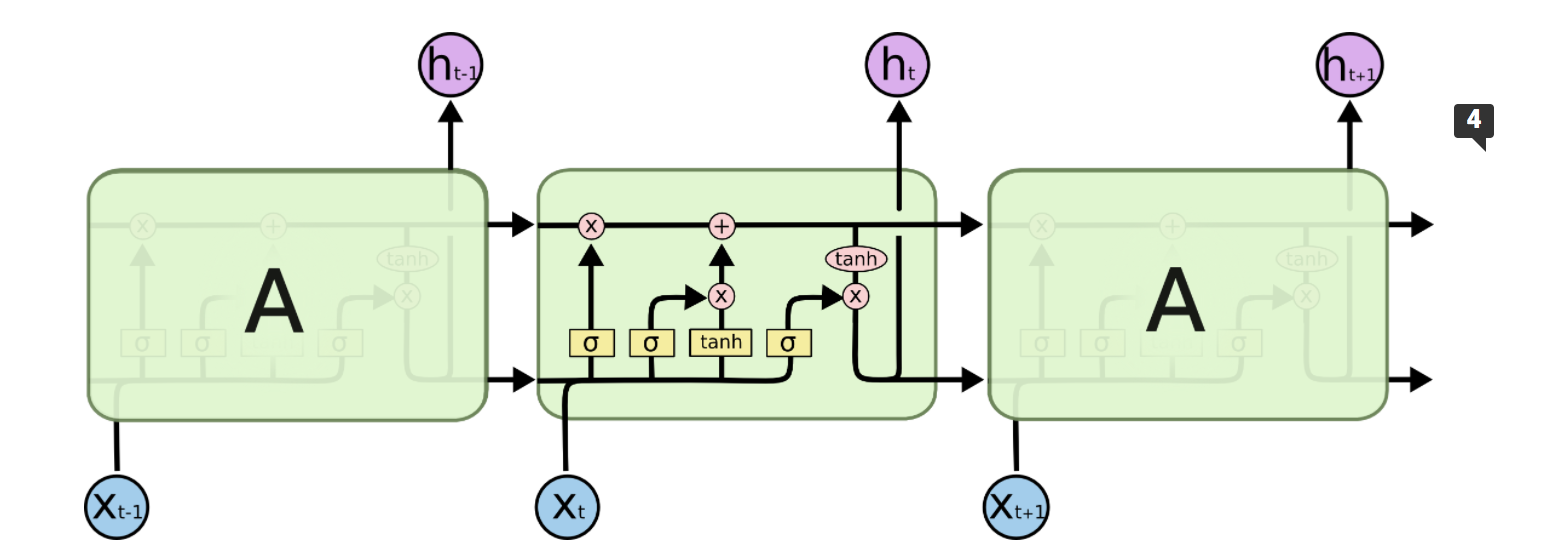
\includegraphics[scale=0.5]{lstm}
\caption{An unrolled diagram of a single-layer LSTM.}
\end{center} 
\end{figure}

\noindent
The mathematical layering of a single-layer LSTM follows:
\begin{align*}
\boldf_t &= \sigma(\boldW_f \cdot [\boldh_{t-1}, \boldx_t] + b_f) \\
\boldi_t &= \sigma(\boldW_i \cdot [\boldh_{t-1}, \boldx_t] + b_i) \\
\tilde{\boldC}_t &= \tanh(\boldW_C \cdot [\boldh_{t-1}, \boldx_t]  + b_C) \\
\boldC_t &= \boldf_t * \boldC_{t-1} + \boldi_t * \tilde{\boldC} \\
\boldo_t &= \sigma(\boldW_o \cdot [\boldh_{t-1}, \boldx_t]  + b_o) \\
\boldh_t &= \boldo_t * \tanh(\boldC_t)
\end{align*}
where $*$ denotes the element-wise multiplication operator. 

For the construction of the overall model to predict the distribution over the next word $\boldx_{t+1}$, we follow the architecture as described by Zaremba et. al in their "large regularized LSTM".  We first encode each word as an embedding $\boldx_t$ of size $d \times 1$.  Then, we pass $\boldx_t$ through a 2-layer LSTM with $l =1500$ hidden units to get an output $\boldo_t$.  For regularization, we then apply dropout with a rate of 0.65 to $\boldo_t$.  Next, we apply a linear transformation to $\boldo_t$ and pass the result through a softmax function to obtain a probability distribution $\boldq_t$ over the next word:
\begin{align*}
\boldq_t = \text{softmax} (W \boldo_t + b)
\end{align*} 
where $W$ is a $\lvert \mathcal{V} \rvert \times l$ matrix and $b$ is a $\lvert \mathcal{V} \rvert \times 1$ vector.  This $\boldq_t$ is then used to calculate the average loss.  We adjust weights to reduce the average loss using different optimizers such as stochastic gradient descent and Adam.  For final comparisons between models of this type, we report perplexity on the test set.           


\section{Experiments}

We performed several experiments to tune the hyper-parameters of our models. In general, the LSTM seemed to perform the best. In-depth explanations of our tuning procedure and associated results can be found in this section. Note that all perplexities reported in table \ref{tab:results} are test set perplexities.

\begin{table}[H]
\centering
\begin{tabular}{llr}
 \toprule
 Model &  & Ppl. \\
 \midrule
 \textsc{Trigram Model} & & 212.48 \\
 \textsc{NNLM + Pretrained Embeddings} & & 164.97 \\
 \textsc{Long Short-Term Memory RNN} & & 139.98 \\
 \bottomrule 
\end{tabular}
\caption{\label{tab:results} Language perplexities of our models.}
\end{table}

\subsection{Trigram Model} 
We chose the parameters $\alpha_i$ by conducting a grid search with stride 0.05 over the space and calculating the validation set perplexity. Our final values are $\alpha = [0.3, 0.5, 0.2]$. We set the initialization value $\beta = 1$ for bigrams and triigrams, and $\beta=0$ for unigrams. (Because there is always at least one word in the training corpus, we won't encounter any undefined behavior without initialization.)

\subsection{Neural Network Language Model}
For the NNLM, we process the data in batches of 20 fragments each, where each fragment is padded to length 32. We train the model for 10 epochs, calculating the validation set accuracy after each epoch and keeping the best model seen thus far (early stopping). We use the Adam optimizer with gradient clipping and initial learning rate $10^{-3}$, halving the learning rate whenever the validation set accuracy does not decrease. The hidden layer size is 200, and the embedding size is 300. Finally, we regularize the learned embeddings by enforcing a maximum norm of 5.  

To improve the performance of our model, we also initialized our embedding weights with the pre-trained GLoVe word vectors with dimension 300. This modification led to a significant improvement in our validation perplexity, decreasing it by around 20 points, with all else held constant.

After experimenting with various $n$-gram sizes, we obtain our best results with $n=5$:
\begin{center}
	\begin{tabular}{ c | c c c c c}
		& n = 3 & n = 4 & n = 5  \\
		\hline
		Val. Perplexity & 171.91 & 166.79 & 164.97
	\end{tabular}
\end{center} 

\subsection{Long Short-Term Memory RNN}
One item we varied in the LSTM RNN was the number of hidden states for the LSTM. Specifically, we looked at differences between the "medium-size" LSTM (650 states) and the "large-size" LSTM (1500 states) proposed by \cite{lstm}. We found that the large-size LSTM took longer to train, but obtained a significantly lower perplexity--the difference is large enough for the large LSTM to be worth it. Here are our best results on both models:
\begin{center}
	\begin{tabular}{ c | c c c c c}
		 & Medium LSTM & Large LSTM  \\
		\hline
		Val. Perplexity & 160.12 & 139.98 
	\end{tabular}
\end{center} 

The second variable that we took into account was the optimization method--either SGD or Adam.  We also varied the \emph{starting} learning rate (STR) for these two methods.  During training, we followed the results in the paper and decreased the learning rate by a factor of 1.2 for each iteration.  Here are our best result under various settings.     

\begin{center}
	\begin{tabular}{ c | c c c c c}
		 & SGD (STR = 1) & SGD (STR = 0.1) & SGD (STR = 0.01)  \\
		\hline
		Val. Perplexity & 203.27 & 156.35 & 183.24 
	\end{tabular}
\end{center} 

\begin{center}
	\begin{tabular}{ c | c c c c c}
		 & Adam (STR = 0.01) & Adam (STR = 0.001)  \\
		\hline
		Val. Perplexity & 152.12 & 139.98 
	\end{tabular}
\end{center} 
Based on these results, we chose to use the Adam optimizer with a starting learning rate of $10^{-3}$.  

Finally, we also experimented with varying the word embedding dimension $d$.  Surprisingly, this had quite a significant effect on the efficacy of the LSTM RNN. Our best model uses an embedding size of 1000, which achieves optimal performance on the validation set:
\begin{center}
	\begin{tabular}{ c | c c c c c}
		 & $d = 100$ & $d = 300$ & $d = 500$ &  $d = 1000$  \\
		\hline
		Val. Perplexity & 189.21 & 151.20 & 143.44  & 139.98 
	\end{tabular}
\end{center}    

\section{Conclusion}
In this practical, we implemented three models to predict the most likely candidates for continuing sentence fragments: A baseline trigram model with linear interpolation, a neural network language model with one hidden layer and one direct connection layer, and a single-layer long short term memory RNN. Our experiments on the Penn Treebank dataset show that the LSTM significantly outperforms the other models, achieving a best perplexity of 139.98 on the test dataset, followed by the NNLM and trigram models, respectively. Future work includes experimenting with ensemble models (e.g., \cite{nnlm} suggest that the trigram and NNLM models are highly complementary, making mistakes on different types of words) and further experimenting with the hidden layer sizes of the NNLM and LSTM.


\bibliography{writeup}
\nocite{*}
\bibliographystyle{apalike}

\end{document}
